\documentclass[12pt,a4paper]{article}
\usepackage{tocloft}
\usepackage{etoolbox}
\usepackage{graphicx}
\usepackage{setspace}
\usepackage{tocloft}
\usepackage{tikz}
\usetikzlibrary{calc}
\usepackage{fancyhdr}
\usepackage{xcolor}
\usepackage{amsmath}
\DeclareMathSizes{12pt}{12pt}{12pt}{8pt}
\makeatletter
\renewcommand{\tagform@}[1]{%
  \maketag@@@{\textnormal{\fontsize{12pt}{12pt}\selectfont(#1)}}%
}
\AtBeginEnvironment{equation}{\fontsize{14}{14}\selectfont}
\AtBeginEnvironment{align}{\fontsize{14}{14}\selectfont}
\makeatother
\renewcommand{\cftsecleader}{\cftdotfill{\cftdotsep}}
\renewcommand{\contentsname}{}
\renewcommand{\listfigurename}{}
\renewcommand{\listtablename}{}
\usepackage[
  top=2.5cm,
  bottom=2.5cm,
  left=2.3cm,
  right=2.5cm
]{geometry}
\usepackage{xeCJK}
\newCJKfontfamily\TraditionalChinese{AR PL KaitiM Big5}
\usepackage{fancyhdr}
\pagestyle{fancy}
\fancyhf{} 
\renewcommand{\headrulewidth}{0pt} 
\fancyfoot[C]{\thepage}       
\usepackage{letltxmacro}
\usepackage{titlesec}


\titleformat{\section}
  {\centering\fontsize{18pt}{18pt}\bfseries} 
  {Chapter \arabic{section}}            
  {1em}                                 
  {}

\titleformat{\subsection}[block]
  {\raggedright\fontsize{16pt}{18pt}\bfseries}
  {\thesubsection}{1em}{}


\titleformat{\subsubsection}[block]
  {\raggedright\fontsize{14pt}{18pt}}
  {\itshape\thesubsubsection}
  {1em}
  {}


\makeatletter
\renewcommand{\sectionmark}[1]{%
  \markright{Chapter \arabic{section}~#1}%
}
\makeatother
\usepackage{setspace}

\usepackage{hyperref}
\hypersetup{
    colorlinks=true,
    citecolor=black,
    linkcolor=black,
    filecolor=black,      
    urlcolor=black,
    pdfborder={0 0 0},
    pdfpagelabels=true,
    plainpages=false
}
\usepackage{cleveref}
\usepackage[sort&compress]{cite}
\usepackage[backend=biber,style=numeric,sorting=none]{biblatex}
\addbibresource{ref.bib}  

\crefformat{equation}{Equation~\textnormal{\fontsize{12}{12}\selectfont(#2#1#3)}}
\Crefformat{equation}{Equation~\textnormal{\fontsize{12}{12}\selectfont(#2#1#3)}}
\crefname{figure}{Figure}{Figures} 
\crefname{table}{Table}{Tables} 
\crefname{algorithm}{Algorithm}{Algorithms} 
\crefname{equation}{Equation}{Equations}
\usepackage{tabularx} 
\renewcommand{\thefigure}{\arabic{section}- \arabic{figure}}
\makeatletter
\@addtoreset{figure}{section}
\makeatother

\renewcommand{\thetable}{\arabic{section}- \arabic{table}}
\makeatletter
\@addtoreset{table}{section}
\makeatother
\renewcommand{\subsectionmark}[1]{}
\renewcommand{\subsubsectionmark}[1]{}

\numberwithin{equation}{section}
\renewcommand{\theequation}{\arabic{section}- \arabic{equation}}
\begin{document}
\linespread{1}
\setlength{\parskip}{1em}


\pagenumbering{Roman}
%英文封面页
\begin{titlepage}
    \centering
    
\includegraphics[width=3cm]{logo_colored.pdf}\\[2.25cm]
    
    {\fontsize{15pt}{18pt}\selectfont\textbf{MACAU UNIVERSITY OF SCIENCE AND TECHNOLOGY}}\\[2.25cm]
    {\fontsize{15pt}{18pt}\selectfont\textbf{School of Computer Science and Engineering\\[0.5cm]
    Faculty of Innovation Engineering}}\\[2.25cm]
    {\fontsize{15pt}{18pt}\selectfont \textbf{Senior Thesis for the Degree of Bachelor of Science}}\\[2.25cm]

    \begin{spacing}{2}
      \noindent
      \hspace*{1cm}
      \begin{minipage}{\dimexpr\textwidth - 1cm\relax}
        {\fontsize{15pt}{18pt}\selectfont
        \begin{tabular}{@{}l l@{}}
          Title: XXX XXX XXX XXX XXX XXX XXX XXX \\
                 XXX XXX XXX XXX XXX XXX XXX XXX XXX ... \\[1cm]
          Student Name \hspace{4pt}: XXX XXX XXX \\[0cm]
          Student No. \hspace{16pt}: XXXXXXXX \\[0.5cm]
          Supervisor \hspace{26pt}: XXX XXX XXX \\
        \end{tabular}
        }
      \end{minipage}
    \end{spacing}

    \vfill
    {\large September, 2024}
\begin{tikzpicture}[remember picture,overlay]
    \draw[line width=3pt]
      ($(current page.north west)+(1cm,-1cm)$) rectangle
      ($(current page.south east)+(-1cm,1cm)$);
\end{tikzpicture}
\end{titlepage}

%中文封面页
\begin{titlepage}
    \centering

    
\includegraphics[width=3cm]{logo.pdf}\\[2.25cm]

    {\fontsize{22pt}{18pt}\selectfont\textbf{澳門科技大學}}\\[2.25cm]

    {\fontsize{16pt}{18pt}\selectfont\textbf{創新工程學院\\[0.75cm]
    計算機科學與工程學院}}\\[0.75cm]

    {\fontsize{16pt}{18pt}\selectfont\textbf{理學學士學位畢業論文}}\\[2.25cm]

    \begin{spacing}{2}
      \noindent
      \hspace*{1cm}
      \begin{minipage}{\dimexpr\textwidth-1cm\relax}
        {\fontsize{15pt}{18pt}\selectfont
        \begin{tabular}{@{}l l@{}}
          論文題目 :  XXX XXX XXX XXX XXX XXX XXX XXX XXX\\
                     XXX XXX XXX XXX XXX XXX XXX XXX XXX\\[1.5cm]
          姓\quad \quad 名 \hspace{4pt}:  XXX XXX XXX\\[0.5cm]
          學\quad \quad 號 \hspace{4pt}:  XXXXXXXX\\[1cm]
          指導老師 \hspace{4pt}:  XXX XXX XXX\\
        \end{tabular}
        }
      \end{minipage}
    \end{spacing}

    \vfill
    {\large 2024 年 9 月}
\begin{tikzpicture}[remember picture,overlay]
    \draw[line width=3pt]
      ($(current page.north west)+(1cm,-1cm)$) rectangle
      ($(current page.south east)+(-1cm,1cm)$);
\end{tikzpicture}
\end{titlepage}

\newgeometry{
  top=3cm,
  bottom=2.5cm,
  left=2.5cm,
  right=2.5cm
}

%英文摘要页
\clearpage
\centering{
\fontsize{18pt}{18pt}{\selectfont {\textbf{\section*{Abstract}}}}
\raggedright
\setlength{\parindent}{2em}
Text text text text text text text text text text text text text text text text text text text text text text text text.

Text text text text text text text text text text text text text text text text text text text text text text text text.

Text text text text text text text text text text text text text text text text text text text text text text text text.

\vspace{2cm}
\noindent % 确保不缩进
{\fontsize{12pt}{6pt}\selectfont\textbf{Keywords:} keyword1; keyword2; keyword3; keyword4; keyword5}
\addcontentsline{toc}{section}{Abstract}

% 中文摘要页
\clearpage
\centering{
\fontsize{18pt}{18pt}{\selectfont{\textbf{\section*{摘要}}}} 
\raggedright                  
\setlength{\parindent}{2em}   
\begin{spacing}{2}
\fontsize{14pt}{18pt}\selectfont{
正文正文正文正文正文正文正文正文正文正文正文正文正文正文正文正文正文正文正文正文正文正文正文正文。

正文正文正文正文正文正文正文正文正文正文正文正文正文正文正文正文正文正文正文正文正文正文正文正文。

正文正文正文正文正文正文正文正文正文正文正文正文正文正文正文正文正文正文正文正文正文正文正文正文。

}
\end{spacing}
\vspace{2cm}
\noindent\fontsize{14pt}{18pt}\selectfont{\textbf{關鍵詞:} 關鍵詞1;關鍵詞2;關鍵詞3;關鍵詞4;關鍵詞5}
\addcontentsline{toc}{section}{摘要}


\renewcommand{\cftsecleader}{\cftdotfill{\cftdotsep}}
\renewcommand{\cftsecfont}{\normalfont\fontsize{12}{14}\selectfont}
\renewcommand{\cftsecpagefont}{\normalfont\fontsize{12}{14}\selectfont}
\renewcommand{\cftsubsecfont}{\normalfont\fontsize{12}{14}\selectfont}
\renewcommand{\cftsubsecpagefont}{\normalfont\fontsize{12}{14}\selectfont}
\renewcommand{\cftfigfont}{\normalfont\fontsize{12}{14}\selectfont}
\renewcommand{\cftfigpagefont}{\normalfont\fontsize{12}{14}\selectfont}
\renewcommand{\cfttabfont}{\normalfont\fontsize{12}{14}\selectfont}
\renewcommand{\cfttabpagefont}{\normalfont\fontsize{12}{14}\selectfont}
\renewcommand{\cftsecpresnum}{Chapter }
\setlength{\cftsecnumwidth}{5.em}
\renewcommand{\cftfigpresnum}{Figure }  
\renewcommand{\cftfignumwidth}{4.5em}     
\renewcommand{\cftfigaftersnum}{}       
\renewcommand{\cfttabpresnum}{Table }   
\renewcommand{\cfttabnumwidth}{4.5em}     
\renewcommand{\cfttabaftersnum}{}     
\renewcommand{\cftsubsubsecpresnum}{\itshape}       % 序号斜体
\renewcommand{\cftsubsubsecnumwidth}{3em}        % 调整序号宽度
\renewcommand{\cftsubsubsecpagefont}{\normalfont\fontsize{12}{14}\selectfont}
\renewcommand{\cftsubsubsecfont}{\normalfont\fontsize{12}{14}\selectfont}

\setlength{\cftsubsubsecindent}{\cftsubsecindent}

\clearpage
\centering{\fontsize{18pt}{18pt}\selectfont\textbf{Table of Contents}}
\addcontentsline{toc}{section}{Table of Contents}
\tableofcontents 

\clearpage
\fontsize{18pt}{18pt}{\selectfont{\textbf{\section*{List of Figures}}}}
\addcontentsline{toc}{section}{List of Figures}  
\listoffigures

\clearpage
\fontsize{18pt}{18pt}{\selectfont{\textbf{\section*{List of Tables}}}}
\addcontentsline{toc}{section}{List of Tables}
\listoftables


\definecolor{mycolor}{RGB}{98, 36, 35}
\fancyhead[C]{%
  \hfill\small \rightmark\\
  \color{mycolor}\rule{\textwidth}{1pt}\\[-9pt]
  \color{mycolor}\rule{\textwidth}{3pt}\\[-2pt]
}
\pagestyle{fancy}

% —— 文档正文 —— 
\clearpage
\pagenumbering{arabic}
\setcounter{page}{1} 
\raggedright                  
\setlength{\parindent}{2em}  
\section{Introduction}
\subsection{Background and motivation}
\hspace{2em}Text text text text text text text text text text text text text text text text text text text text text.

Text text text text text text text text text text text text text text text text text text text text text.

Text text text text text text text text text text text text text text text text text text text text text.
\subsection{Thesis organization}
\hspace{2em}Chapter 2, text text text text text text text text text text text text text text text text text text text. 

Chapter 3, text text text text text text text text text text text text text text text text text text text. 

Chapter 4, text text text text text text text text text text text text text text text text text text text. 

Chapter 5, text text text text text text text text text text text text text text text text text text text. 

Chapter 6 concludes the thesis, text text text text text text text text text text text
text text text.

\clearpage
\section{Title2}
\hspace{2em}Text text text text text text text text text text text text text text text text text text text text text
\subsection{Section 1}
\hspace{2em}Text text text text text text text text text text text text text text text text text text text text text \cite{1}.

\subsubsection{\textit{Sub Section 1}}
\hspace{2em}Text text text text text text text text text text text text text text text text text text text text text, as shown in \cref{fig:2- 1}.

\begin{figure}[h]
    \centering
    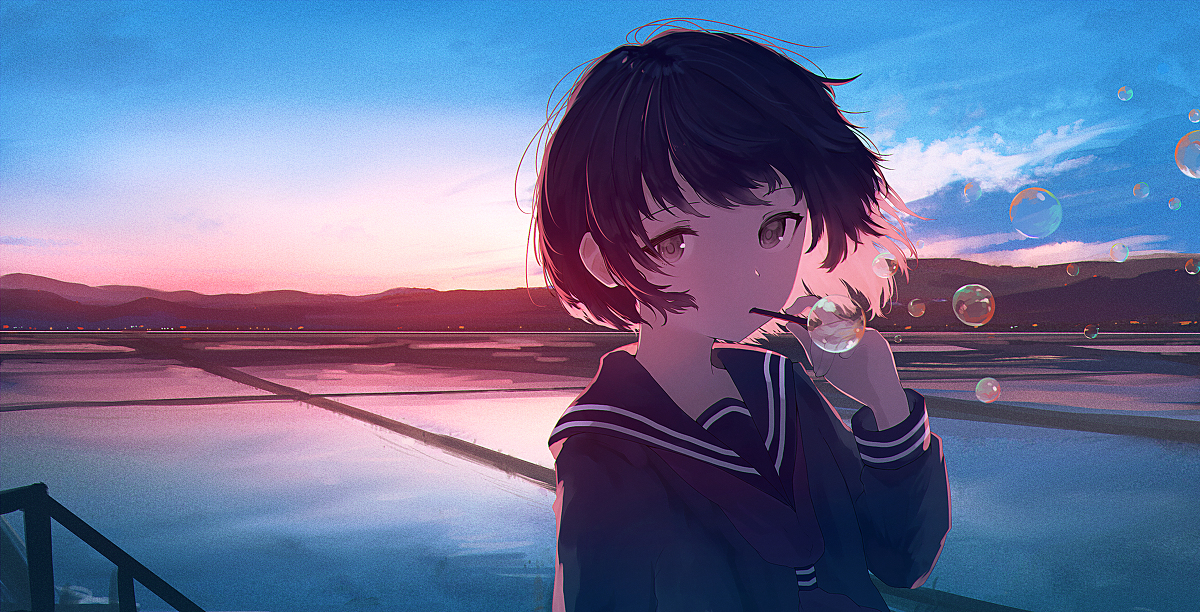
\includegraphics[width=1\textwidth, height=0.8\textwidth]{Fig example.png}
    \caption{Figure title}
    \label{fig:2- 1}
\end{figure}

\subsubsection{\textit{Sub Section 2}}
\hspace{2em}Text text text text text text text text text text text text text text text text text text text text text, as shown in \cref{tab:2-1}.

\renewcommand{\arraystretch}{4}
\begin{table}[htbp]
  \centering 
  \label{tab:2-1}
  \begin{tabular}{|p{5cm}|p{5cm}|p{5cm}|}
    \hline
     &  &  \\
    \hline
     &  &  \\
    \hline
     &  &  \\
    \hline
  \end{tabular}
  \caption{Table title}
\end{table}

\subsubsection{\textit{Sub Section 3}}
\hspace{2em}Text text text text text text text text text text text text text text text text text text text text text, as shown in \cref{Eq (2- 1)}.
\begin{align}
    \label{Eq (2- 1)}
    y = x + 1
\end{align}

\subsection{Section 2}
\hspace{2em}Text text text text text text text text text text text text text text text text text text text text text \cite{2}.

\subsection{Section 3}
\hspace{2em}Text text text text text text text text text text text text text text text text text text text text text \cite{3}.


\section{Title3}
\hspace{2em}Text text text text text text text text text text text text text text text text text text text text text.

\subsection{Section 1}
\hspace{2em}Text text text text text text text text text text text text text text text text text text text text text \cite{4}.

\subsubsection{\textit{Sub Section 1}}
\hspace{2em}Text text text text text text text text text text text text text text text text text text text text text, as shown in \cref{fig:3- 1}.
\begin{figure}[h]
    \centering
    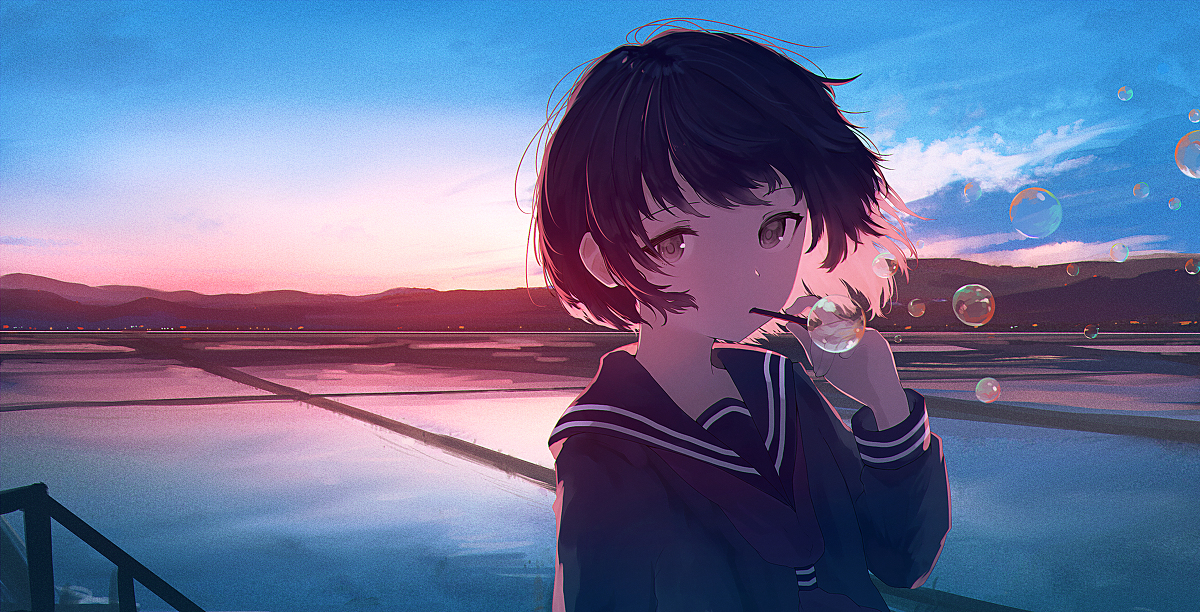
\includegraphics[width=0.8\textwidth, height=0.8\textwidth]{Fig example.png}
    \caption{Figure title}
    \label{fig:3- 1}
\end{figure}

\section{Title4}
\hspace{2em}Text text text text text text text text text text text text text text text text text text text text text.
\subsection{Section 1}
Text text text text text text text text text text text text text text text text text text text text text \cite{5}.
\subsubsection{\textit{Sub Section 1}}
\hspace{2em}Text text text text text text text text text text text text text text text text text text text text text, as shown in \cref{fig:4- 1}.
\begin{figure}[h]
    \centering
    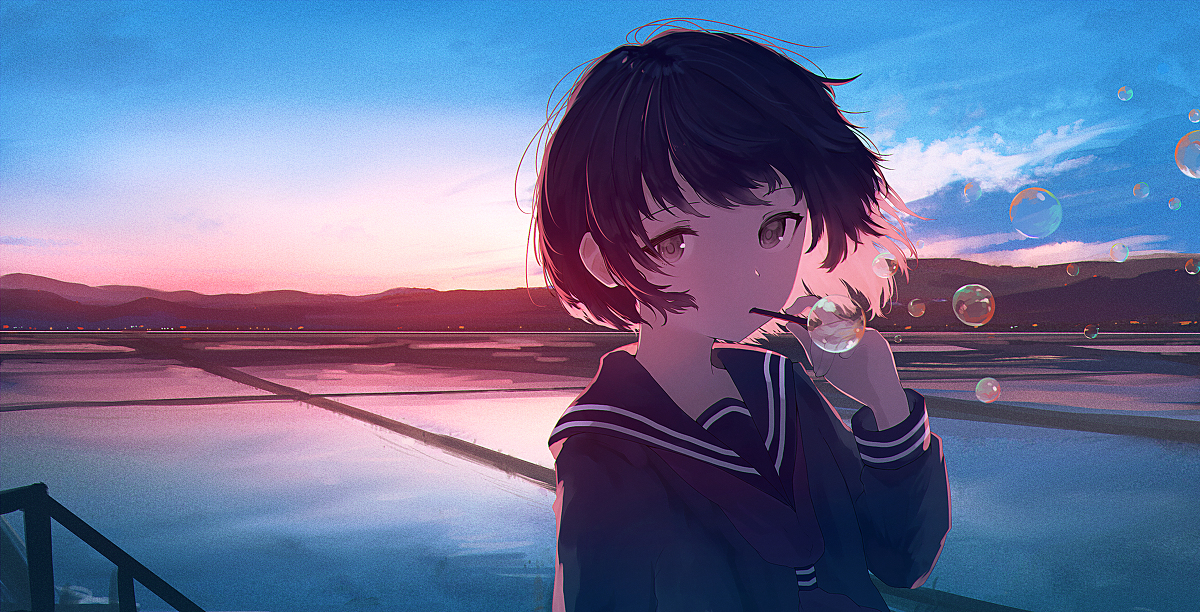
\includegraphics[width=0.8\textwidth, height=0.8\textwidth]{Fig example.png}
    \caption{Figure title}
    \label{fig:4- 1}
\end{figure}

\section{Title5}
\hspace{2em}Text text text text text text text text text text text text text text text text text text text text text.
\subsection{Section 1}
\hspace{2em}Text text text text text text text text text text text text text text text text text text text text text \cite{6}.
\subsubsection{\textit{Sub Section 1}}
\hspace{2em}Text text text text text text text text text text text text text text text text text text text text text, as shown in \cref{fig:5- 1}.
\begin{figure}[h]
    \centering
    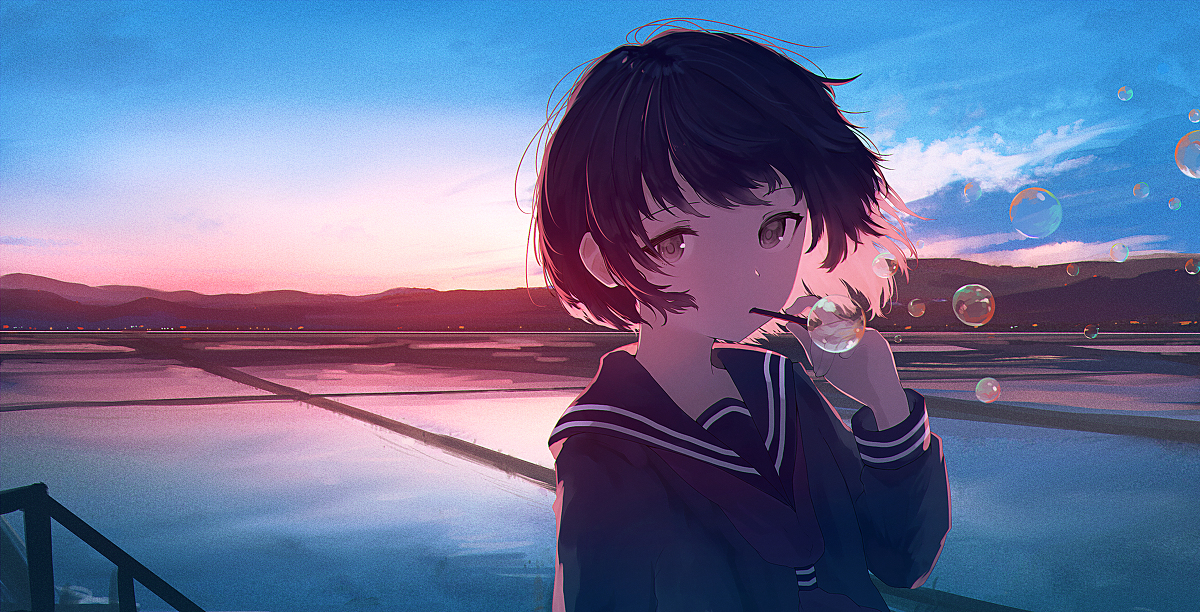
\includegraphics[width=0.8\textwidth, height=0.8\textwidth]{Fig example.png}
    \caption{Figure title}
    \label{fig:5- 1}
\end{figure}

\section{Conclusion}
\subsection{Conclusion}
\hspace{2em}Text text text text text text text text text text text text text text text text text text text text text.
\subsection{Future work}
\hspace{2em}Text text text text text text text text text text text text text text text text text text text text text.

\clearpage
\addcontentsline{toc}{section}{References}
\markright{References}
\printbibliography

\clearpage
\addcontentsline{toc}{section}{Appendix}
\markright{Appendix}
\section*{Appendix}

\clearpage
\addcontentsline{toc}{section}{Resume}
\markright{Resume}
\section*{Resume}
\textbf{\subsection*{1. Resume}}
Name: XXX XXX XXX\\ [0.5cm]
\noindent Gender: Male/Female\\[0.5cm]
\noindent Email: xxx@xxx.xxx\\[0.5cm]
\noindent Education:\\[0.5cm]
0000 ~ 0000, High School, School Name.\\[0.5cm]
0000 ~ 0000, Bachelor of Science, University Name.\\[0.5cm]
…\\[0.5cm]
\noindent Awards:\\[0.5cm]
…\\[0.5cm]
\noindent Work experience:\\[0.5cm]
…\\[1cm]

\textbf{\subsection*{2. Publications}}

\renewcommand{\refname}{}
\patchcmd{\thebibliography}{\section*{\refname}}{}{}{}
\begin{thebibliography}{99}  
    \bibitem{ref1}paper 1.
    \bibitem{ref2}paper 2.
    \bibitem{ref3}paper 3.
\end{thebibliography}

\clearpage
\addcontentsline{toc}{section}{Acknowledgements}
\markright{Acknowledgements}
\section*{Acknowledgements}
\hspace{2em}Text text text text text text text text text text text text text text text text text text text text text.

Text text text text text text text text text text text text text text text text text text text text text.

Text text text text text text text text text text text text text text text text text text text text text.
\end{document}

